  
\documentclass[titlepage]{article}
\usepackage[utf8]{inputenc}
\usepackage{amsmath}
\usepackage{tcolorbox}
\usepackage{amssymb}
\usepackage{amsthm}
\usepackage{empheq}
\usepackage{hyperref}
\usepackage{listings}
\usepackage{xcolor}
\usepackage{float}
\usepackage{xparse}
\usepackage{mathtools}
\DeclarePairedDelimiter{\ceil}{\lceil}{\rceil}
\usepackage[
top    = 2.50cm,
bottom = 2.50cm,
left   = 2.75cm,
right  = 2.75cm]{geometry}
\usepackage{fancyhdr}
\pagestyle{fancy}
\lhead{AICC 2}
\rhead{EPFL/Alp Ozen}

\newtheorem{remark}{Remark}[section]
\newtheorem{theorem}{Theorem}[section]
\newtheorem{lemma}[theorem]{Lemma}
\newtheorem{prop}{[Proposition]}
\newtheorem{definition}{Definition}
\newtheorem{question}{Question}

\newcommand{\interior}[1]{%
  {\kern0pt#1}^{\mathrm{o}}%
}
\newcommand{\Rn}{\mathbb{R}^n}
\newcommand{\Rm}{\mathbb{R}^m}
\newcommand{\R}{\mathbb{R}}

\title{\textbf{AICC 2 - Bixio Rimoldi}}
\author{Alp Ozen}
\date{Spring 2019}
\newtheorem{example}{Example}[section]
\newtheorem{axiom}{Axiom}
\newtheorem{cor}{Corollary}

\begin{document}

\maketitle
\tableofcontents
\clearpage

\section{Week 2}

\subsection{Entropy}
We begin by defining \textbf{entropy} as Shannon put it:

\begin{definition}\textbf{Entropy}

Note that this definition assumes base $2$ aka. binary.
$$ H(s) = - \sum_{s \in A} p(s)\log_{2}p(s) \ \text{A being our alpahabet aka. sample space}$$
and thus an equivalent definition is:
$$ H(s) = E[-\log_{2}p(s)]$$
And similarly, Shannon defines information as:
$$-\log_{2}p(s)$$
\end{definition}

For a random distribution we get:

\begin{example}
$$\forall x \in A \ p(x) = \frac{1}{|A|}, \ -\log_{2}p(s) = \log_{2}|A|$$
Hence the entropy function $H(s) = E[\log_{2}|A|]} = \underbrace{\log_{2}|A|}_{\text{do the algebra}}$
\end{example}

And now we present the \textbf{information theory inequality}

\begin{definition}\textbf{IT inequality}
$$ \log_{b}r \leq (r-1)\log_{b}(e)$$
\end{definition}

\begin{proof}
Given that $$\ln(r) \leq (r-1)$$ and that $$ ln(r) = \frac{\log_{b}(r)}{\log_{b}(e)}$$ we are done.
\end{proof}

And now we present the Entropy bound theorem:
\begin{theorem}
$$S \in A \ 0 \leq H(S) \leq \log|A|$$ 
\end{theorem}

\begin{proof}
We only show the RHS as the LHS is more or less trivial. 
Our goal is to show:

\begin{align*}
    \text{need to reach} H(s) - \log|A| \leq 0 \\
    E[-\log p(s)] - \log |A|\\
    = E[\log \frac{1}{p(s)|A|}]\\
    = \sum_{s\in A}p(s)(\log \frac{1}{p(s)|A|})\\
    \leq \underbrace{log(e)\sum[\frac{1}{|A|} - p(s)]}_{\text{using IT ineq.}} = 0
\end{align*}
\end{proof}
\subsection{Source coding}
A code is said to have a prefix if:
\begin{definition}\textbf{Prefix of a code}
\\

For some sequence of characters $a_{1}a_{2}\ldots a_{n}$ and $b_{1}b_{2}\ldots b_{m}$ with $n \leq m$ we have $a_{1}a_{2}\ldots a_{n} =  b_{1}b_{2}\ldots b_{n}$
\end{definition}

A \textbf{prefix free code} also known as \textbf{instantaneouss code} is one that has no prefixes. And now we come to the important \textbf{Kraft-McMillan} result:

\begin{theorem}
If a $D-ary$ code is uniquely decodable, then it satisfies:

$$ D^{-l_{1}} + \ldots + D^{-l_{m}} \leq 1 $$
\textcolor{red}{Note that there are non-instantaneous codes that stil satisfy this inequality. By the same token, by the contrapositive, we have that if a code does not satisfy the inequality, then there exists no prefix-free version of it.}
\end{theorem}

We now define the \textbf{average codeword length}

\begin{definition}\textbf{average codeword length}
$$ L(S,R) = \sum_{s \in A} p_{S}(s)L(R(s)) \ \text{where $L$ represents length}$$
\end{definition}

Given this definition, another important result is:

\begin{theorem} \textbf{Lower bound and Upper bound for average optimal codeword length}
$$H_{d}(S) \leq L(S,R) \leq H_{d}(S) + 1$$
\end{theorem}

This result becomes a useful tool once we realize the similarity in the definitions as below:

\begin{align*}
    H(S) = - \sum p(s)\log p(s)\\
    L(S,R) = \sum p(s)L(R(s))
\end{align*}

Given this, \textit{Shannon - Fano} realized that we may define a code of length $\ceil*{\log_{D} p(s)}$
This satisfies the Kraft inequality hence we now have a method of obtaining uniquely decodable code. 
\\

But as it turns out, Huffman was the first to actually find out how one finds an optimal code. We list our alphabet with probability in increasing order. Then, if say we are working in base 2, we simply continuously combine the smallest probabilities and build our branches from them. Hence, as below, we have that a Huffman code isn't always unique:

\begin{figure}[H]
    \centering
    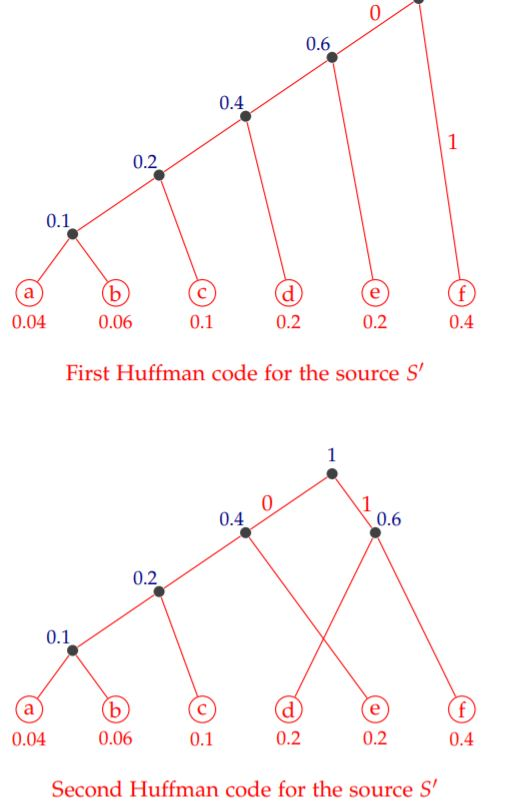
\includegraphics[scale = 0.3]{src/huff.JPG}
    \caption{Huffman codes}
    \label{fig:my_label}
\end{figure}

\section{Week 3}
We now define conditional entropy(the intuition for this being, we want to mesure uncertainty given knowledge of something else) as follows:

\begin{definition}
$$H(X|Y) := - \sum p(x|y)\log p(x|y)$$
\end{definition}

And the law of \textbf{total probability}

\begin{theorem}
Imagine we take a sample space with some subset $A$ and cut it into 3 disjoint units $B_{i}$. Now we may describe the set $A$ as $A = (B_{1} \cap A) \cup (B_{2} \cap A) \cup (B_{3} \cap A)$ This is equivalent to now saying:

$$p(A) = p(B_{1} \cap A) + p(B_{2} \cap A) + p(B_{3} \cap A) $$
Which in terms of conditional probability is $$p(A) = p(A|B_{1})p(B_{1}) + p(A|B_{2})p(B_{2}) + p(A|B_{3})p(B_{3})$$
\end{theorem}

And another useful theorem is:

\begin{theorem}
$$H(s_{1},s_{2},\ldots,s_{n}) \leq H(s_{1}) + H(s_{2}) + \ldots + H(s_{n})$$
with equality iff the $s_{i}$ are independent. 
\end{theorem}

A similar result now is the chain rule of conditional entropy.
\begin{theorem}\textbf{Conditional entropy chain rule}
$$H(S_{1},S_{2},\ldots,S_{n}) = H(S_{1}) + H(S_{2}|S_{1}) + \ldots + H(S_{n}|S_{1},\ldots,S_{n-1})$$
\end{theorem}

To clarify the notation used above, when we write $P_{X_{1}}, \ldots, X_{n}(x_{1},\ldots, x_{n})$ we interpret each comma as an intersection$\cap$

And we now introduce what it means for a source to be \textbf{regular}

\begin{definition}\textbf{Regular source}
\\
A source is regular if
\begin{align*}
    H(S) := \lim_{n\to\infty} H(S_{n})\\
    H^{*}(S) := \lim_{n \to \infty} H(S_{n}|S_{1},S_{2},\ldots,S_{n-1})
\end{align*}

exist and are finite. 
\end{definition}

Now it should be intuitively obvious that conditioning would reduce entropy. Lets prove it.

\begin{theorem}
$$H(X|Y) \leq H(X)$$
\end{theorem}

\begin{proof}
\begin{align*}
    E(\log\frac{1}{p(X|Y)}) + E(\log p(X))\\
    = E(\log\frac{p(X)}{p(X|Y)})\\
    = E(\log\frac{p(X)p(Y)}{p(X|Y)p(Y)})\\
    \leq (\frac{p(X)p(Y)}{p(X\cap Y) - 1}\log(e)
    \leq 0
\end{align*}
\end{proof}

\section{Week 4}

We begin by making an important distinction in the definition of conditional entropy.

\begin{definition}\textbf{Conditional entropy given $Y=y$}
\\
We define this as:
$$H(X|Y=y) = - \sum_{x \in (\cdot | y)} P(x|y)\log P(x|y)$$
\end{definition}

Given this definition, the more general definition of conditional entropy is:

\begin{definition}
$$H(X|Y) = - \sum P(y)H(X|Y=y) $$
\end{definition}

And we now introduce a \textbf{stationary source}

\begin{definition}\textbf{Stationary source}
\\
A source is stationary if $\forall n,k$ the blocks $S_{1}, \ldots, S_{n}$ and $S_{n+1}, \ldots, S_{k}$ have the same statistic that is:
\begin{align*}
    P_{s_{1}} = P_{s_{i}}
\end{align*}

\end{definition}


\begin{theorem}
All stationary sources are regular. 
\end{theorem}

And now we come to another intuitive result:
\begin{theorem}
$$H^{*}(S) = \lim_{N\to \infty}\frac{H(S^{n})}{n}$$
\end{theorem}

The intuition for this result is that the entropy rate is inversely proportional to how much information we have. That is the more variables we know, the more we reduce entropy. 

We now consider an instructive example
\begin{example}
Suppose we are given two machines $M_{1}$ and $M_{2}$ that produce 3 bits. $M_{1}$ produces any number between 0 and 7 with equal chance and $M_{2}$ produces a number in range 0 to 3 with equal chance. We ask then, what is the probability distribution of the sequence $s_{1}\ldots s_{n}$

Well noticing that this is equal to finding 

$$ P(S_{1}\ldots S_{n})=P(S_{1}\ldots S_{n}|S_{0})P(S_{0}) = P(S_{1}\ldots S_{n}|S_{0})P(S_{0} = M_{1}) + P(S_{1}\ldots S_{n}|S_{0})P(S_{0} = M_{2})$$

We obtain:
$$P(S_{1}\ldots S_{n}) = \[   \left\{
\begin{array}{ll}
     \frac{1}{8^{n}}\frac{1}{2} + \frac{1}{4^{n}}\frac{1}{2} \text{if} s_{1}\ldots s_{n} \in \{0,\ldots,3\}^{n}\\
     \frac{1}{8^{n}}\frac{1}{2}
\end{array} 
\right. \]$$
\end{example}

\section{Week 5}
This week, we introduce cryptography. 
We begin by listing the most common attack methods.

\begin{itemize}
    \item \textbf{Chosen-plaintext attack}: The attacker is able to obtain a ciphertext for any arbitrary plaintext. Thus to obtain the key, one might encode every single letter. 
    \item \textbf{Known-plaintext attack}: Attacker has access to both ciphertext and plaintext.
    \item \textbf{Ciphertext-only attack}: Attacker has access to a set of ciphertexts. A possible attack method is to use a frequency analysis. 
\end{itemize}

We now introduce the vigenere cipher.
\begin{definition}\textbf{Vigenere's cipher}
Vigenere cipher makes use of the Caesar cipher. Suppose we are given a 7 letter plaintext. The sender chooses another keyword of 7 letters. This we call the key. Then encryption is done using the lookup table below.

\begin{figure}[H]
    \centering
    
\includegraphics[scale = 0.6]{src/vigenere.png}
    \caption{Lookup table}
    \label{fig:my_label}
\end{figure}

As an example suppose our plaintext is "hello", an example key is "abcde". Thus the encrypted word would become "hffos"
\end{definition}

Now we introduce a very strong type of secrecy. 

\begin{definition}\textbf{Perfect secrecy}
A cryptosystem has perfect secrecy if the plaintext and ciphertext are statistically independent. 
\end{definition}

Given this perfect secrecy implies:
\begin{theorem}
H(T) \leq H(K)
\end{theorem}

And now we present an instructive example on how one would try to crack vigenere given we have the ciphertext and a portion of the plaintext.

\clearpage

\begin{example}\textbf{Cracking Vigenere}
\begin{figure}[H]
    \centering
    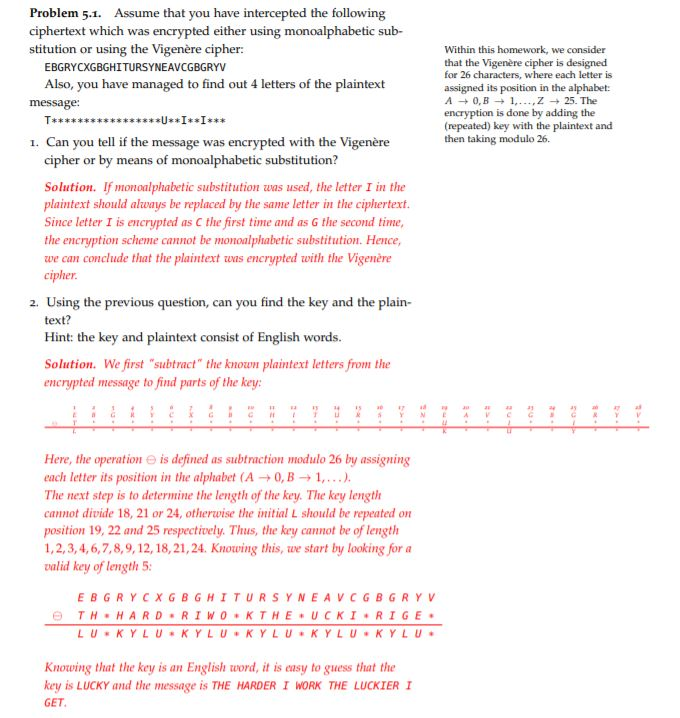
\includegraphics{src/vig.JPG}

    \label{fig:my_label}
\end{figure}
\end{example}

We know present a method used to verify the correctness of data sent.
\begin{example}
Suppose we want to send an IBAN number over the net. It is possible that for some reason, during transmission, two digits of the credit card get flipped. We need a system to verify the correctness of information sent. Here's how we proceed:
\begin{itemize}
    \item concatenate 00 to the end of the IBAN number.
    \item mod out by 97, fix this as $a$.
    \item now our key $k$ is found as $98-a=k$
    \item concatenate $k$ to the end of the IBAN number removing the 00 and now send it to the recipient
    \item receiver mods out by 97, if result is congruent to 1, success.
\end{itemize}

Here is why this works:
Given $x \equiv a \mod{97}$
\begin{align*}
    x^{\prime} \equiv x + (98 - a) \mod{97}\\
    x^{\prime} \equiv x + 98 - x \mod{97}\\
    x^{\prime} \equiv 98 \mod{97} \equiv 1 \mod{97}\\
\end{align*}

Yet another proof is to show the following implication:
$$100n_{97} - 100\Tilde{n}_{97} \equiv 0_{97} \implies a=b \text{where a,b are changed digits}$$

Now our above equality simplifies to:

$$10^{k+1}a+10^{k}b - 10^{k+1}b - 10^{k}a = 10^{k}(9a-9b)$$
Now since all expressions in the above equations have an inverse as we are in base 97, we get:
$$ (a-b)_{97} \equiv 0_{97}$$
which is only the case if $a=b$
\end{example}

A neat modulo trick is presented below.

\begin{theorem}
For some number $a = d_{n}\ldots d_{1}$ in base 10 we have that:
$$a \bmod{11} = \sum_{i}^{k}10^{i}d_{i} \bmod{11} = \underbrace{\sum_{i}^{k}-1^{i}d_{i}}_{10\equiv-1\bmod{11}} \bmod{11}$$
\end{theorem}

\section{Week 6}

We present some definitions and theorems which we later use to define certain structures in $\mathbb{R}$.

\begin{definition}\textbf{Ring}
A ring is a triple $(R,\alpha,\mu)$ such that the following hold:
\\

$R,\alpha$ known as the 'addition' on $R$ is an abelian group 
\\

$R, \mu$ is both associative and right-left distributive over addition
\\

If it is also the case that $R/{e_{\alpha}}$ is an abelian group, our ring is called a \textit{commutative ring with unity}

\end{definition}
\\

\begin{theorem}
The inverse of an element under any binary relation is unique.
\end{theorem}

\begin{proof}
Let $ab = e$ and also $ac=e$. Then $abb=acb$ which simplifies to $eb=ec=b=c$
\end{proof}

\begin{theorem}
Within $\mathbb{Z} / m\mathbb{Z}$ the following theorems are equivalent:
\\

$\forall a \in \mathbb{Z}, \exists a^{-1}$
\\

$f:\forall a \in \mathbb{Z} \to \forall a \in \mathbb{Z}$ is a bijection
\\

$ax=b$ has a unique solution 

\end{theorem}

\begin{theorem}
Some $[a]_{m}$ has a multiplicative inverse iff $gcd(a,m)=1$
\end{theorem}

Given the above, something that easily follows is:

\begin{theorem}
If $p$ is prime, then all $a \in \mathbb{Z}/p\mathbb{Z}$ have a multiplicative inverse 
\end{theorem}

\begin{remark}\textbf{Useful facts about the gcd}
$$gcd(a,b) = gcd(b,a-kb)=gcd(\pm a, \pm b)$$
\end{remark}

We now present the Euclidian algorithm used to find $gcd(a,b)$ in pseudocode and explain why it works.


\begin{lstlisting}
if(a<b) return:
gcd(b,a);
else if(b=0) return:
a;
else return:
gcd(b,a\% b);
\end{lstlisting}

\begin{theorem}\textbf{Bezout's theorem}
$$gcd(a,b) = au + bv \ a,b \in \mathbb{Z}$$
\end{theorem}

We now ask given the above theorem, how we may find the $u$ and $v$. Well let's take an example:
\begin{example}
Find the $u,v$ for $gcd(56,15)$.
By normal Euclidian algorithm, it turns out that $gcd(56,15) = 1$ Our steps in finding this are:
\begin{align*}
    56 = 15(3) + 11\\
    15 = 11(1) + 4\\
    11 = 4(2) + 3\\
    4 = 3(1) + 1\\
    3 = 1(3) + 0
\end{align*}

Now notice how we from the above already have:
$$56 - 15(3) = 11 \ 4 - 3(1)=1$$
Hence all that's left to do now is make $4 - 3(1)=1$ top and work our way down.
\begin{align*}
    4 - 3(1) = 1\\
    4 -  11 + 4(2)\\
    4(3) - 11\\
    (15 - 11(1))3 - 11\\
    15(3) - 11(4)\\
    15(3) - (56-15(3))4\\
    (-4)56 + (12)15 
\end{align*}

\end{example}

\begin{lemma}
$$gcd(a,m) = 1 \iff \ \exists u,v \ 1 = au + mv$$
\end{lemma}




We now explore some notation relating to modular classes:
\begin{itemize}
    \item $[a]_{m} :=$ congruence class $\bmod{m}$
    \item $\mathbb{Z} / m\mathbb{Z} :=$ all congruence classes $\bmod{m}$
    \item The structure $<\mathbb{R} / m\mathbb{Z}, + , \cdot>$ is an abelian ring 
    \item By $\mathbb{Z} / m\mathbb{Z}^{*}$ we denote the set where an inverse exists. 
\end{itemize}

\begin{definition}\textbf{Totient function}
 $\phi (x): \mathbb{Z} \to \mathbb{N}$ computes the number of integers that are relatively prime to $x$.
\end{definition}

\begin{lemma}
When $p$ is prime, $\phi(p) = p-1$
\end{lemma}

\begin{remark}
The cardinality of $\mathbb{Z} / m\mathbb{Z}^{*}$ is $\phi(m)$
\end{remark}

\begin{remark}
$$\phi (p^{k}) = p^{k} - p^{k-1}$$ for some prime $p$
\end{remark}

Yet another super useful result that appears in RSA encryption is the following:
\begin{remark}
Let $p$ and $q$ be prime numbers, we ask what is $\phi (pq)$
$$\phi (pq) = pq - (p + q -1) = (p-1)(q-1) = \phi (p) \phi (q)$$
which follows from the fact that the numbers relatively prime to $pq$ are:
$$ \[   \left\{
\begin{array}{ll}
     p,2p,\ldots, qp\\
     q,2q,\ldots,(p-1)q
\end{array} 
\right. \]$$
\end{remark}

Finally we define perhaps one of the most fundemental mathematical structures, that is an isomorphism.

\begin{definition}\textbf{Isomorpishm}
\\

 Let $(H_{1},\cdot_{1})$ and $(H_{2},\cdot_{2})$ be two structures. An isomorphism $\phi$ from $H_{1}$ to $H_{2}$ is bijection such that:
 $$\forall a,b \in H_{1} \ \phi(a\cdot_{1} b) = \phi(a)\cdot_{2} \phi(b)$$
\end{definition}



\section{Useful links}
Amazing YouTube playlist: \hyperlink{ https://www.youtube.com/playlist?list=PLE125425EC837021F}{YT Information Theory playlist}



\end{document} 
